\chapter{Systeme}
\label{cha:systeme}
Die Entscheidungsgrundlage 

\section{MobileIron}

\subsection {Allgemein} 
Das Unternehmen MobileIron ist ein US-amerikanisches Unternehmen mit Hauptsitz in Kalifornien welches im Jahr 2007 gegründet wurde. MobileIron hat sich von Anfang an auf die Verwaltung von mobilen Endgeräten im Enterprise Umfeld spezialisiert. Das Unternhemen wurde 2017 im siebten Jahr in folge als Leader im Magic Quadrant von der Gartner Inc. neben VMWare, IBM und BlackBerry für MDM/EMM Suites gekürt. Das Softwareentwicklungsunternehmen bietet in Ihrem Produktportfolio verschiedene Bring Your Own Device Pakete mit zahlreichen Funktionen an. 
\subsection {Kompatibilität}
Der Hersteller MobileIron unterstützt in seinen Lösungen die  mobilen Endgeräte Apple iOS, Google Android und Microsofts Windows Phone. Zusätzlich können klassische Desktop Geräte mit den Betriebssystemen Microsoft Windows (ab 8.1) und Apple OS X (ab 10.9)  verwaltet werden. 
\subsection {Paketmodelle}
MobileIron bietet die drei verschiedenen Bundles „EMM Silver“, „EMM Gold“ oder „EMM Platinum“ seiner Bring Your Own Device Lösung an.
Das Basispaket „EMM Silver“ beinhaltet die Komponenten „Core“ „Sentry „und „Apps@Work“. Das Paket „EMM Gold“ ist um die Module „Email+“, „Docs@Work“ und „Web@Work“ erweitert. Durch die Wahl des Platinum Pakets ergänzt sich dieses wiederum um „Help@Work“, „Tunnel“, „MobileIron Monitor“ und „ServiceConnect-Integration“.

\begin{figure}[hbt]
\centering
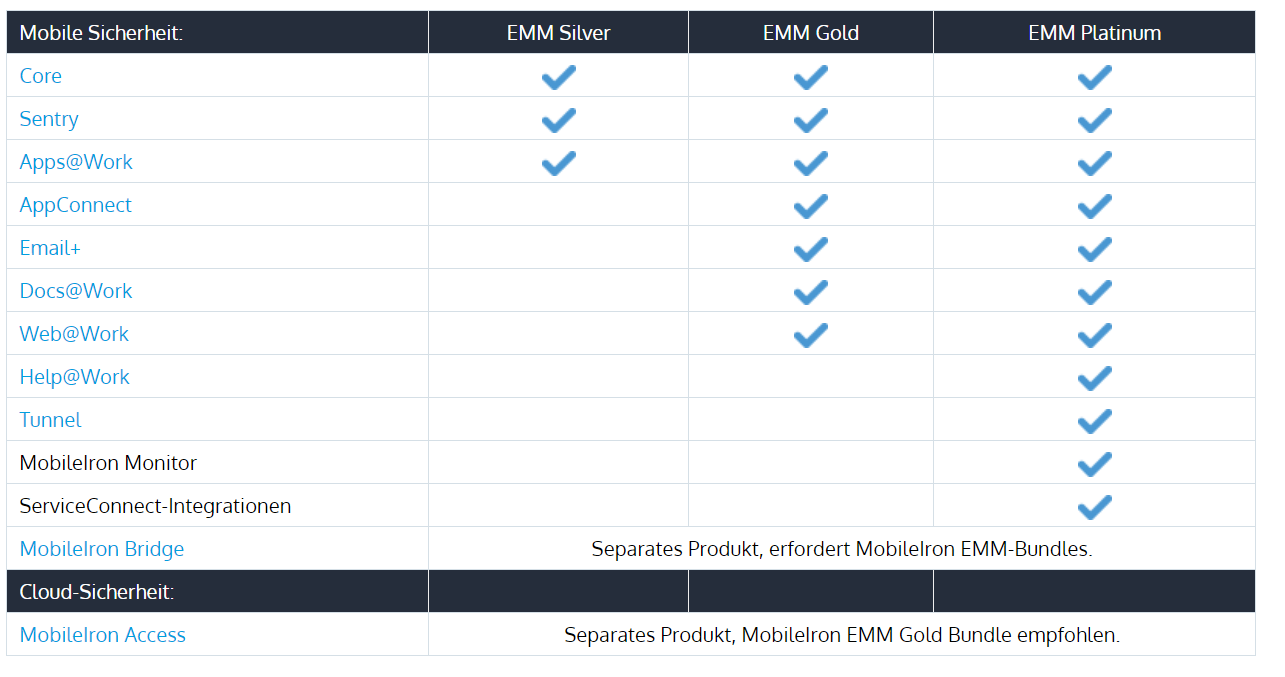
\includegraphics[width=0.95\textwidth]{Bilder/mi_1.png} 
\caption{Mobile Iron Paketmodelle}\label{fig:MobIro1}
\end{figure}

\subsection {Pakete}
\subsubsection {Core}
Das Paket Core ist das zentrale Modul, welches das IT-Backend des Unternehmens einbindet. Hierüber können die erforderlichen Sicherheits- und Verwaltungsrichtlinien der mobilen Endgeräte definiert und verwaltet werden. Über die  API Schnittstellen des Cores kann man komfortabel Erweiterungen nutzen. Im Fokus des Cores stehen jedoch die das MDM, MAM und MCM. Der Core bietet für die Administratoren zusätzliche Analyse- und Auswerungsfunktionen. So kann beispielsweise der von den Endgeräten produzierten Netzwerktraffic ausgewertet werden um Infrastrukturprobleme zu lokalisieren. Durch die Möglichkeit Dachboards-Widgets anzulegen kann der Administrator das System und die verschiedenen Gerätestatus komfortabel überblicken. 
\subsubsection {Sentry}
Die Komponente Sentry ist das Inline-Gateway, das den gesamten Netzwerkverkehr zwischen den Mobilgeräten und dem Unternehmensbackend verschlüsselt, verwaltet und sichert. Sentry setzt die in der Core Komponente definierten Sicherheitsrichtlinien um. Sentry kann beispielsweise E-Mail Anhänge verschlüsseln, sodass nicht autorisierte Applikationen auf diese Daten nicht zugreifen können. 

\subsubsection {Apps@Work}
Apps@Work ist ein unternhemenseigener App Store, indem sowohl eigenentwickelte als auch öffentliche, freigegebene Anwendungen für die Benutzer bereitgestellt werden können. Über diesen Weg können Administratoren schnell auswählen, welche Anwendungen erforderlich, zulässig oder verboten sind. 
\subsubsection {AppConnect}
Durch AppConnect können auf den Endgeräten installierte Applikationen geschützt werden. Hierbei werden die entsprechenden Anwendungen in Containern gekapselt und sind somit vor unberechtigtem Zugriff geschützt. Alle in Containern befindlichen Apps können durch eine Tunnellösung miteinander kommunizieren um beispielsweise die Funktion eines Single Sign Ons bereitzustellen oder den Austausch von Daten bereitzustellen. 
\subsubsection {Email+}
Die gesamte Unternehmenskommunikation über mobile Endgeräte kann über die App Email+ abgewickelt werden. Die Anwendung stellt E-Mails, Kalender und Kontakte dar. Dabei findet eine strikte Trennung von beruflichen und privaten Inhalten statt. 
\subsubsection {Docs@Work}
Die Anwendung Docs@Work ist ein Tool um Dokumente auf Endgeräten zu verwalten und zu editieren. Hierbei ist ein besonderes Augenmerk auf die Synchronisation und Sicherung der Daten gelegt. 
\subsubsection {Web@Work}
Der Unternehmensbrowser Web@Works bietet dem Benutzer die Möglichkeit auf intern betriebene Webseiten oder Webapplikationen zuzugreifen.  Dabei ist die komplette Kommunikation verschlüsselt. Über verschiedene Benutzergruppen können die  Zugriffsrechte  auf die verschiedenen internen Webressourcen reglementiert werden. 
\subsubsection {Help@Work}
Help@Work ist ein Tool für die Fehlerdiagnose. Neben dem Abfragen und Übertragen von Ereignisprotokollen kann unter dem Betriebssystem Android sogar ein Remotezugriff für den IT-Support gewährt werden. 
\subsubsection {Tunnel}
Der Tunnel von MobileIron bietet die Möglichkeit die Netzwerkkommunikationen einzelner Apps durch eine VPN Verbindung auf der Basis von Zertifikaten zu schützen.

\subsection {Abrechnungsmodell}

Je nach Tarifplänen bzw. Paketangeboten werden neben den genannten Grundfunktionen weitere Features unterstützt. Das Unternehmen selbst betreibt ein sehr flexibles Abrechnungsmodell, welches auf jegliche Bedürfnisse des Endkunden angepasst werden kann. Dabei kann beispielsweise zwischen einer Lizenzierung pro Benutzer (maximal 3 Endgeräte) oder einem Lizenzierungsmodell je nach Endgerät gewählt werden. Neben der Kaufoption von Lizenzen auf Lebenszeit wird auch ein Abonnement angeboten. Neben der klassischen Installation innerhalb des eigenen Netzwerks betreibt MobileIron auch eine eigene Cloud die für die Bereitstellung der Services genutzt werden kann. Falls sich der Endkunde für die Cloudlösung entscheidet kann direkt ein erweiterter Support (SLA) dazu gebucht werden. Für die Installation auf einem eigenen System kann hierbei nur zwischen einem Standard- und Premiumsupport unterschieden werden.  

\begin{figure}[hbt]
\centering
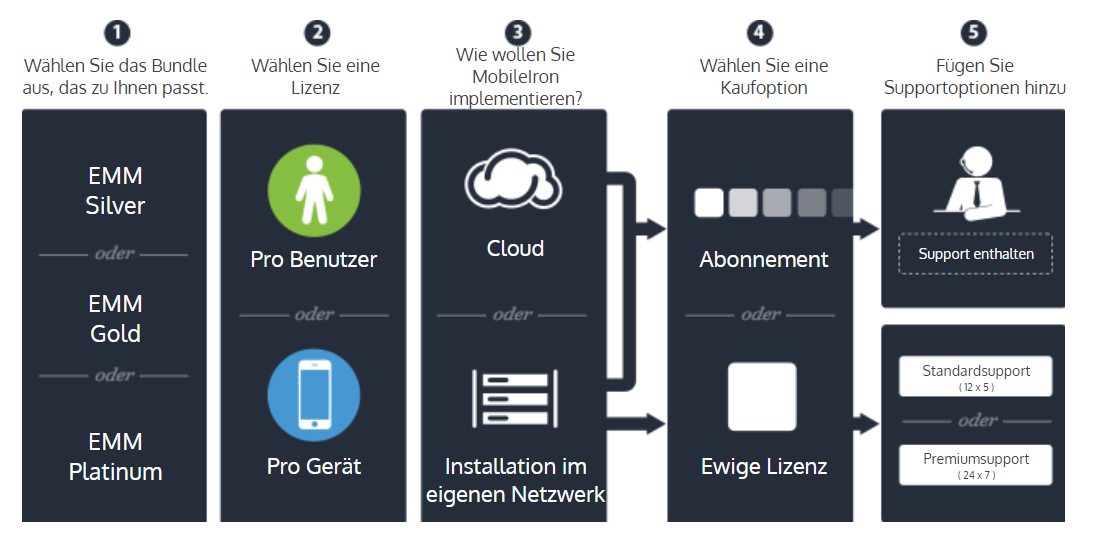
\includegraphics[width=0.95\textwidth]{Bilder/mi_2.png} 
\caption{Mobile Iron Abrechnungsmodell}\label{fig:MobIro2}
\end{figure}

\newpage

% --------------------------------------------------------------------------------------------------------------------------
\section{Samsung Knox}
% --------------------------------------------------------------------------------------------------------------------------

\subsection{Allgemein}\label{sub:Allgemein}
Das weltbekannte Unternehmen Samsung hat ebenfalls an einer Sicherheitslösung für die Mobilnutzung im Unternehmen gearbeitet. Als Produkt ist Samsung Knox, in Anlehnung an Hochsicherheitsstützpunkt Fort Knox, im Portfolio von Samsung zu finden.
Ist man Besitzer aktueller Samsung-Geräten findet man die Applikation \textit{Sicherer Ordner}\footnote{Sicherer Ordner löste am 19. Dezember 2017 den Vorgänger MyKnox ab \cite{sam2017b} }als vorinstallierte Standardsoftware vor. Mit Öffnen dieser App können, nach Eingabe eines benutzerdefinierten Sicherheitsverfahren, verschiedene Einstellungen getätigt werden. Es ist möglich Dateien oder Apps in diesen \flqq sicheren Ordner\frqq  zu verschieben. Sogar Apps die vorher nicht auf dem Smartphone vorhanden sind, können direkt vom Store geladen und installiert werden.Theoretisch wäre dieser Lösungsansatz genau richtig für die Verwendung von BYOD und zusätzlich sogar kostenlos. Dennoch wäre dies nicht umsetzbar im Enterprise-Umfeld.

Um den Anforderungen an eine BYOD-Lösung der Loco AG gerecht zu werden, benötigt es eine MDM-Möglichkeit. Dafür muss die IT-Administration, die Möglichkeit haben die eingesetzten Geräte zu verwalten und somit an die firmeninternen Sicherheitsanforderungen anzupassen. Eine mögliche Lösung bietet Samsung mit der kostenpflichtigen Variante Samsung Knox Premium, die im Folgenden nach dem Kriterienkatalog belichtet werden soll. 

\subsection{Knox-Plattform}
Die Knox-Plattform ist die technische Umsetzung in Hardware und Software, welche standardmäßig in Samsunggeräten vorzufinden ist. Das Sicherheitsverfahren der Knox-Plattform besteht, wie in \cref{fig:SamKno1} sichtbar, aus fünf Komponenten.
\begin{figure}[hbt]
\centering
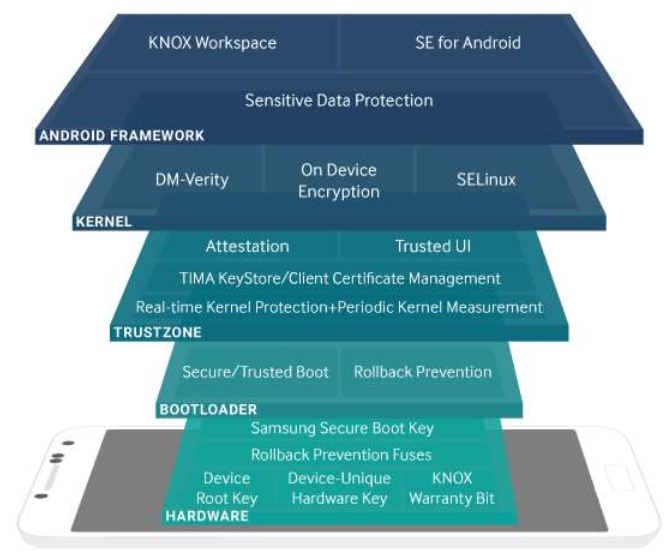
\includegraphics[width=1\textwidth]{Bilder/sk_1}
\caption{Samsung Knox Security Solutions Layers}\label{fig:SamKno1}
\end{figure}
Die Knox-Plattform setzt bereits in der Hardware-Ebene ein. Der Prozessor ist die Steuereinheit auf dem bekanntlich das entsprechende Betriebssystem und die Applikationen laufen. Modi bestimmen welche Priorität, welcher Software oder Applikation zugeschrieben werden. So laufen vom Benutzer installierte Apps im Modus \textit{user mode} und haben somit keinen direkten Zugriff auf die Hardware, das Betriebssystem oder auf andere Apps. Die \textit{ARM TrustZone} beschreibt eine Prozessorarchitektur, die von der Knox-Plattform verwendet wird. Hierbei werden die Modi in \textit{Worlds} eingeteilt. Zum einen die \textit{Normal World}, auf dem standardmäßig alle installierte Software landet und die \textit{Secure World}, die durch kryptographische Methoden gesichert wird und sich in einer isolierten Hardwareumgebung befindet, und somit für das geschäftliche Nutzen des Smartphones eingesetzt werden soll.\footnote{Vgl. \cite{sam2017c}}

Beim Anschalten eines Gerätes, startet für gewöhnlich die Boot-Chain (zu dt. Hochfahrkette), die nacheinander die Softwarekomponenten startet. Zum Auschließen von Fremd- oder Schadsoftware wird ein \textit{Secure Boot} ausgeführt. Jede Komponente in der Kette prüft die Integrität der vorangehenden Komponente durch Abfrage einer Signatur. Wenn die Verifikation einer Signatur fehlschlägt, also eine mögliche Modifikation stattgefunden ist, wird entweder der weitere Startvorgang verhindert oder es wird der \textit{Knox Warranty Fuse} ausgelöst, welcher prüft ob das Gerät vorher jemals einen unzulässigen Status hatte. Allerdings stößt \textit{Secure Boot} beim Unterscheiden von akzeptierten Versionen an seine Grenzen, da er neue Versionen einer Software direkt als gültig sieht. Hierzu wird der \textit{Trusted Boot} hinzugezogen, welcher beim Durchlaufen der Boot-Chain den Hash der nächsten Komponente in die TrustZone Secure World lädt.\footnote{Vgl. \cite{sam2017d} } Es kann also Software nur genehmigt und gestartet werden, die auch als erlaubt in der TrustZone stehen. Das Unternehmen hat die Kontrolle darüber, welche Versionen von welcher Software, sei es öffentlichzugängliche oder eigenentwickelte Software, verwendet werden sollen. 

Denkbar wäre natürlich, dass während der Laufzeit, also nachdem die Überprüfung auf richtige Software, eine fälschliche Modifikation stattfindet. Um dem gegenzuwirken nutzt Samsung Knox die \textit{Real-Time Kernel Protection} (RKP) um Veränderungen am Kernel zu verhindern und die \textit{Periodic Kernel Measurements} (PKM) zum periodischen Überprüfen der Integrität des Kernels.\footnote{Vgl. \cite{sam2017d} }. Diese beiden Sicherheitsverfahren spielen sich ebenfalls in der \textit{TrustZone Secure World} ab und sind somit isoliert und nicht zugänglich vom Kernel.
Weitere integrierte Verfahren in die Knox-Plattform sind Google DM Verify, genauer beschrieben in \cite{Goo2017a}, welches überprüft ob das Gerät sich im selben Zustand befindet, wie beim letzten Start und SE for Android, genauer beschrieben in \cite{Goo2017b}, dass \textit{mandatory access control} (MAC) über alle Prozesse vollzieht.
\subsection{Knox Solutions}
\subsubsection{Knox Configure}

\subsubsection{Knox Mobile Enrollment}
Um ein EMM-System aufzubauen, ist es notwendig, dass die Mitarbeiter auch Samsung Knox auf ihrem Endgerät installiert haben. Dies findet häufig per Download vom \textit{Google Play store} statt, dem darauf folgenden Autentifizieren und weiteren Einstellen des Workspaces auf die Unternehmensrichtlinien. 
Damit diese manuelle Installation durch den Mitarbeiter vermieden und damit Fehler vermieden werden können, gibt es das \textit{Knox Mobile Enrollment} (KME). Ein Enrollment durch KME funktioniert durch einen Link, der je nach Unternehmensbelangen, bspw. per E-Mail oder Interner Webseite an den Mitarbeiter vermittelt wird. Nachdem dieser Link aufgerufen wird, werden nach entsprechenden Autentifizierungsmaßnahmen, alle Einstellungen und Applikationen automatisch konfiguriert.

\subsubsection{Knox Manage}

\subsubsection{Knox Workspace}
Samsung's Knox Workspace entspricht dem in \cref{sub:Allgemein} beschriebenen \flqq sicheren Ordner\frqq in der Enterprise-Welt. Das heißt, es exisitiert eine Containerlösung für Mobilgeräte, ersichtlich in \cref{fig:SamKno2}, auf dem geschäftliche Applikationen und Daten von den eigenen getrennt werden können. Es ist nicht möglich außerhalb des Workspaces auf Daten oder Applikationen innerhalb zuzugreifen, aber von innerhalb auf außerhalb. So ist es beispielsweise nicht möglich Bilder, die innerhalb des Workspaces gemacht wurden, außerhalb in der App Galerie anzuschauen.
\begin{figure}[hbt]
\centering
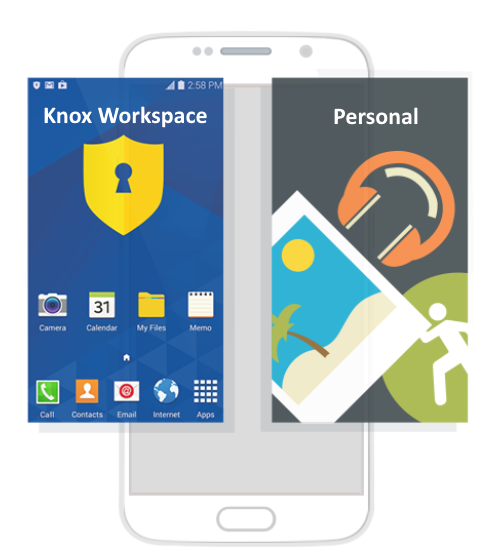
\includegraphics[width=0.5\textwidth]{Bilder/sk_2}
\caption{Samsung Workspace Container}\label{fig:SamKno2}
\end{figure}

Um die Container des Samsungs Workspace zu verwalten, wird das \textit{Mobile Container Management} verwendet. Hierbei können Authentifizierungsmöglichkeiten, Datensicherheit,  VPN, Blacklisting und viele weitere Features, die wie andere EMM Lösungen nutzen gemanaged werden.

Um Zugang zum Workspace zu bekommen wird ein doppeltes Autentifizierungsverfahren verwendet. Hierzu muss der Nutzer zuerst den Fingerabdruck oder wenn es das Gerät zulässt, den Iris-Scanner nutzen und als zweites PIN oder Password eingeben. Erst dann ist ihm Zugriff gewährt.
Andersrum ist es so möglich den Workplace als Autentifizerung zu nutzen. Hierzu gibt es beispielsweise die Möglichkeit per \textit{Near Field Communication} (NFC) das Smartphone als SmartCard agieren zu lassen und so beispielsweise den Zugriff in Sicherheitsbereiche oder Accounts zu gewähren.
Welche Methodiken schlussendlich, wie genutzt werden sollen, kann das IT Managagement des MCM's je nach Sicherheitsanforderung im Unternehmen anpassen.

\subsubsection{Samsung E-FOTA}
Mit der Samsung E-FOTA-Lösung können alle Geräte mit demselben Betriebssystem betrieben werden.


\subsection{Kompatibilität}
Um Knox Workspace, Knox Mobile Enrollment und Samsung E-FOTA zu nutzen benötigt es eine geeignete EMM-Lösung. In \cref{fig:SamKno3} sind einige EMM Lösungen und deren Kompatibilität mit den Samsung Knox Paketen aufgezeigt.
\begin{figure}[hbt]
\centering
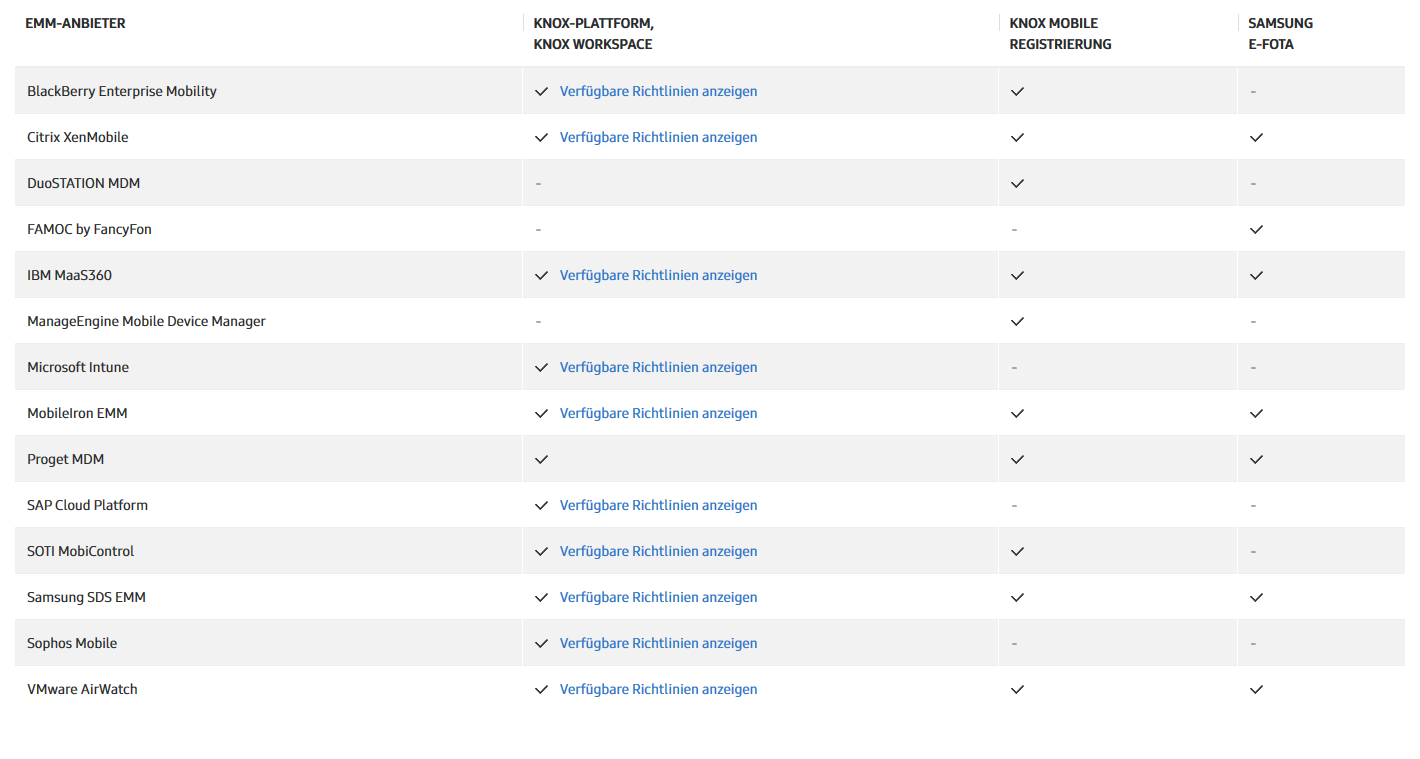
\includegraphics[width=1\textwidth]{Bilder/sk_3}
\caption{Unterstützte EMM-Dienstleister}\label{fig:SamKno3}
\end{figure}

\subsection{Kosten}

\newpage

% --------------------------------------------------------------------------------------------------------------------------
\section{VM AirWatch}
% --------------------------------------------------------------------------------------------------------------------------
\subsection{Paketmodelle}


\subsection{Workspace ONE}
Vmware Workspace ONE ist eine Enterprise-Plattform, die einen digitalen Workspace zu den entsprechenden und geforderten Bedürfnissen bietet. Dieser bietet dem Nutzer 

\subsection{Workspace Horizon}

\subsection{Kosten}
\begin{figure}[hbt]
\centering
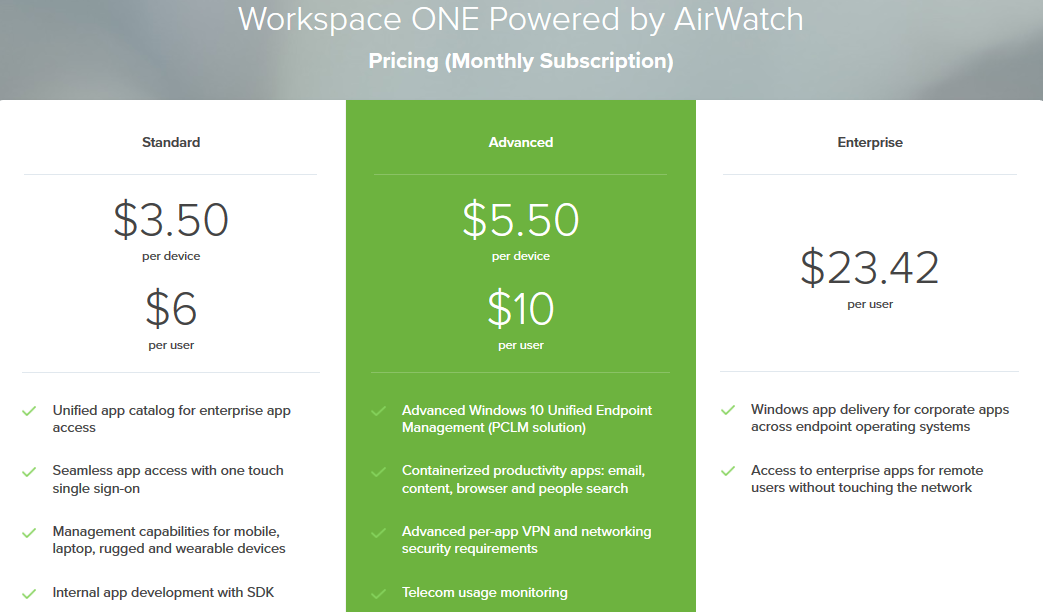
\includegraphics[width=0.95\textwidth]{Bilder/aw_1.png} 
\caption{AirWatch Kosten nach Paket}\label{fig:AirWat1}
\end{figure}























